 \section{Experiments}
\label{sec:experiments}
\begin{figure}
    \centering
    \begin{subfigure}[b]{0.23\textwidth} 
        \captionsetup{justification=centering}
        \begin{center}
        \hspace*{-0.3cm} 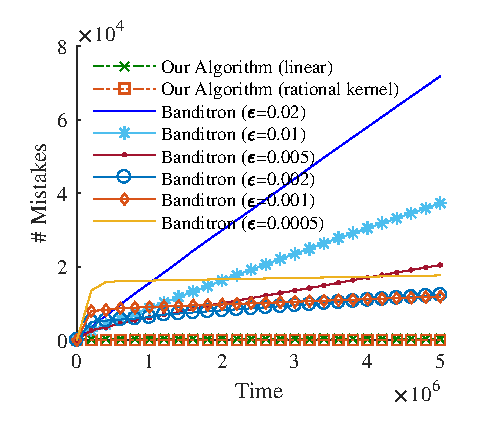
\includegraphics[width=1.15\textwidth, trim={0, 0.1cm, 0, 0}, clip]{figures/strong3}
        \caption{Strongly separable case}
        \end{center}
    \end{subfigure}
    \hfill
    \begin{subfigure}[b]{0.23\textwidth} 
        \captionsetup{justification=centering}
        \centering
        \hspace*{-0.3cm}  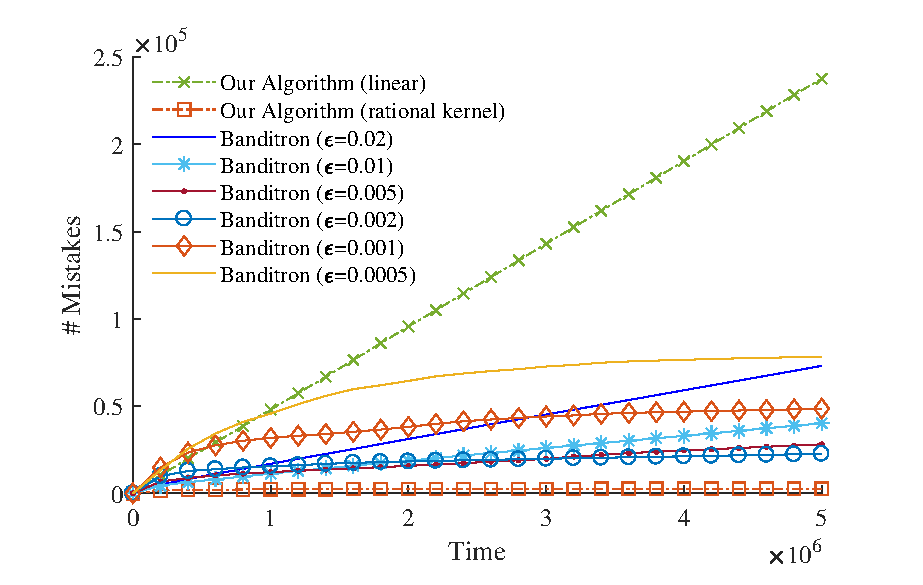
\includegraphics[width=1.15\textwidth, trim={0, 0.1cm, 0, 0}, clip]{figures/weak3}
        \caption{Weakly separable case}
    \end{subfigure}
    \vspace*{-0.2cm}
    \caption{Comparison between our algorithm and Banditron with different exploration parameter $\epsilon$ under $\gamma=0.05$ and $K=3$. }
    %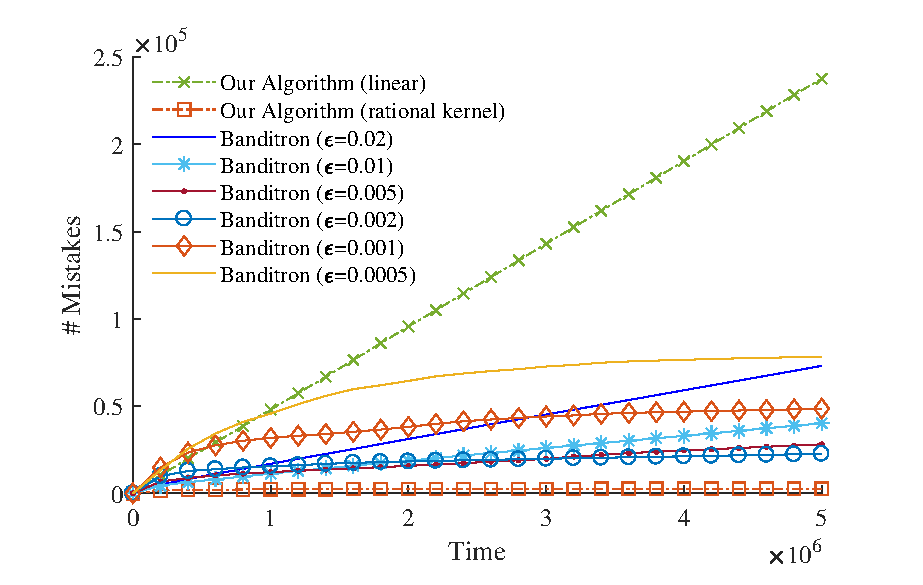
\includegraphics[width=0.25\textwidth]{figures/weak3}
    \label{fig:both}
\end{figure}

We compare our algorithm with \textsc{Banditron} empirically to show that our kernelized bandit algorithm can have significant advantage over \textsc{Banditron} is the separable case. 

We generate strongly and weakly separable samples with $K=3$ in a similar sense those in Figure~\ref{figure:weakly-linearly-separable-examples-with-margin}. They are originally generated in a $d=2$ plate, and then lifted to $d=3$ by adding a constant feature. We provide the figures of their exact look in Appendix~\ref{sec:supp-to-experiment}. Different from Figure~\ref{figure:weakly-linearly-separable-examples-with-margin}, the three classes are non-uniform and imbanlanced: class 1 occupies a smaller sector between $-15^\circ$ and $15^\circ$, while class 2 and class 3 occupy $[15^\circ, 180^\circ]$ and $[-180^\circ, -15^\circ]$ respectively. On the other hand, $80\%$ of data comes from class 1, while $10\%$ comes from class 2 and 3 each. 

In real world, data can often be non-uniform and imbalanced. We demonstrate that \textsc{Banditron} is weak especially under these situations, while our algorithm still performs well.

We choose sample size as $5\times 10^6$ and margin as $\gamma=0.05$ (in both strongly weakly separable cases). All results are averaged over $20$ runs. 

We plot the number of mistakes against time in Figure~\ref{fig:both}. We can see there is indeed a dilemma for \textsc{Banditron}: when picking a relatively large exploration rate, it suffers from the cost of continuous exploration; when picking a relatively small exploration rate, it cannot adapt its model quickly enough (this problem exacerbates when a majority class occupies a small region, like class 1). Striking a balance between the two extremes leads to the $\sqrt{T}$ mistake bound. On the contrary, our algorithm makes significant progress on every mistake it makes, leading to a finite mistake bound.  